
\documentclass{subfiles}

\begin{document}

\section{Problem}\label{sec:Problem}
\par FW LiDAR systems have been available for a number of years but there still very few uses of FW LiDAR data. NERC-ARF has been acquiring airborne data for the UK and overseas since 2010 and it has more than 100 clients of new and archived data. Many clients request FW LiDAR data to be acquired, but despite the significant number of requests, the majority of research still only uses discrete LIDAR. Some of the factors regarding this slow intakes are:
\begin{itemize}
	\item Typically FW datasets are 5 – 10 times larger than discrete data, with data sizes in the range of 50GB – 2.5TB for a single area of interest. NERC-ARF's datasets are up to 100GB each because most clients are research institutes but for commercial purposes each FW dataset is a couple of TB.
	\item Existing workflows are only able to work with the discrete data since the increased amount of information recorded within the FW LiDAR makes handling the quantity of data very challenging.
\end{itemize}

\newpage

\section {Aims and Objectives}\label{sec:AimsObjectives}
	
\par This thesis explores visualisation and data-understanding for FW LIDAR systems and the overarching aim is to increase the accessibility FW LiDAR in remote forest surveying. The objectives are listed in Table \ref{tab:Objectives} and they are associated with the Sections that tackle them.

\begin{table}[!htbp]
	% increase table row spacing, adjust to taste
	\renewcommand{\arraystretch}{1.3}
	% if using array.sty, it might be a good idea to tweak the value of
	% \extrarowheight as needed to properly center the text within the cells
	
	\centering
	% Some packages, such as MDW tools, offer better commands for making tables
	% than the plain LaTeX2e tabular which is used here.
	\begin{tabular}{|P{.1\textwidth}|P{.7\textwidth}|P{.2\textwidth}|}	
		\hline
		\textbf{No.} &	\textbf{Objective} &	\textbf{Related Chapters}  \\
		\hlinewd{1.5pt}
		1 &	Enable forestry experts with no computer science expertise to visualise and work with the FW LiDAR data.  &	\ref{Visualisations} \\	
		\hline
		2 &	Enable forest understanding through 3D visualisations of FW LiDAR data. &	\ref{Visualisations}  \\
		\hline
		3 &	Improve and optimise visualisations of FW LiDAR data and hyperspectral images. &	\ref{Optimisations} \& \ref{Alignment}  \\
		\hline
		4 &	Enable browsing of very large scale datasets and spectral bands in an efficient manner. &	\ref{Optimisations} \& \ref{Alignment}   \\
		\hline
		5 &	Investigate data structures for faster iso-surface extraction of large volumetric datasets and efficient management of voxels. &	\ref{Optimisations} \\	
		\hline
		6 &Estimate tree coverage and investigate the potential of integrating multiple remote sensing datasets in forestry. &	\ref{Alignment}  \\
		\hline
		7 &	Dead tree detection in comparison to human detection and remote surveying with FW LiDAR that will benefits biodiversity management. &	\ref{Classifications}  \\
		\hline
		8 &	Research whether terrain classification can be improved by the inference of high quality 3D information. &	\ref{Classifications}  \\
		\hline
		
		\hline
	\end{tabular}
	\caption{Values of divisible sides}
	\label{tab:Objectives}
\end{table}
\newpage
\section{Thesis Overview}\label{PipeLine}


\par To address the limitations of existing workflows for using with FW data we developed the open source software DASOS (named after $\delta \alpha \sigma o \varsigma$, which means forest in Greek) and novel algorithms that allow users, without computer science expertise, to work with and visualise large volumes of FW LiDAR data. Our open source software DASOS aims to remove the barriers preventing the use of FW LiDAR. Its contributions, and those of the new representations of the FW LiDAR, are demonstrated in three applications:

\begin{itemize}
\item Firstly, foresters can exploit their domain expertise to derive a wealth of information by observing the FW LiDAR data. We therefore improve visualisations for deriving information directly from the data, thus reducing travelling time and the associated expenses of getting into the forests. This cost includes appropriate cars and sometimes helicopters depending on the accessibility of the forests. While previous work on FW LiDAR visualisation talks about point cloud visualisation \cite{Isenburg2012Pulsewaves} and transparent voxels \cite{Persson2005}, DASOS is able to extract a 3D surfaces from the scanned area. This research further introduces new data structures for accelerating the surface extraction processed. 

\item Secondly, a fast way of aligning the FW LiDAR with Remotely Sensed Images has been developed in DASOS. Subsequently, by generating tree coverage maps, it has been shown that the combination of these datasets confers better remote survey results \cite{Miltiadou2015}.


\item Finally, DASOS allows the generation of feature vectors characterising objects like trees. An example usage of this information is characterising dead standing Eucalyptuses, which as explained at Section \ref{sec:forestMonitoring} are extremely beneficial for managing biodiversity in native Australian forests. 

\end{itemize}



\par To sum up, FW LiDAR has great potential to improving automated surveying accuracy and consequently reduce the expensive fieldwork conducted in forestry. This research has already started to have an impact in the FW LiDAR community. DASOS is now used at Interpine Group Ltd, a world leading Forestry Company in New Zealand, I occasionally receive emails with questions or suggestion about the software and according to github the visitors are slowly increasing; during the last forty days, there were six unique visitors and one cloner (Figure \ref{fig:githupStatistics}).


 	\begin{figure} [h!]
 		\centering
 		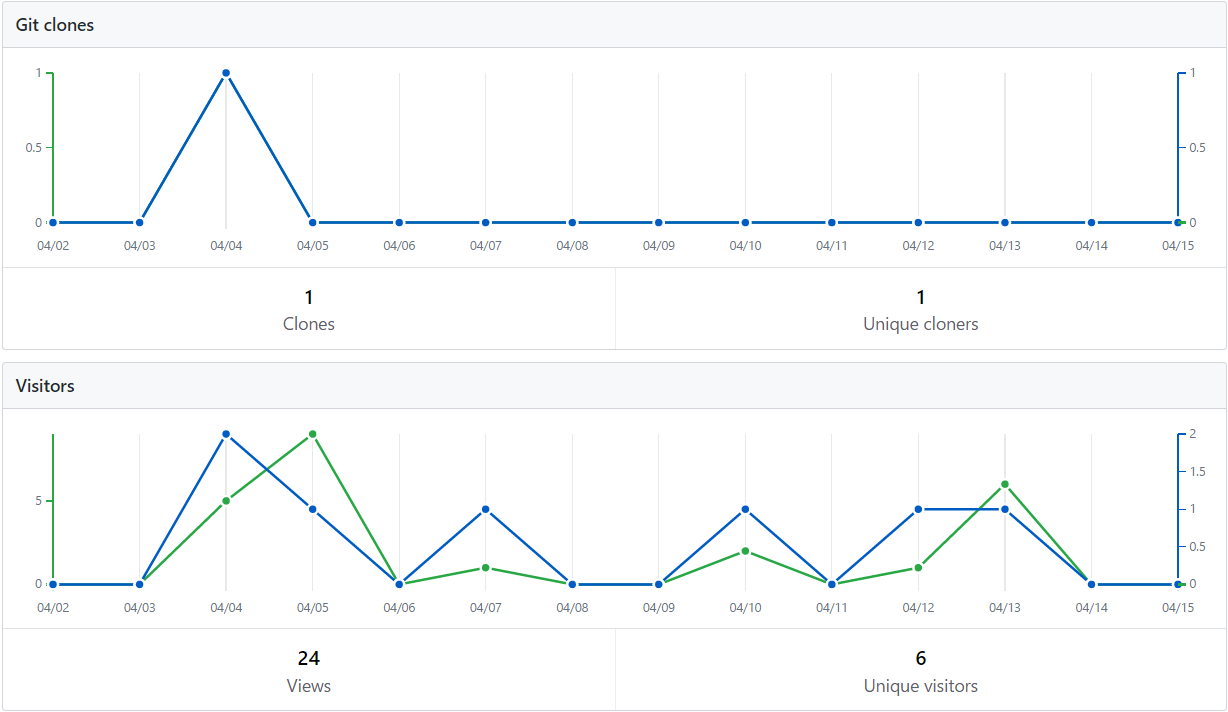
\includegraphics[width=\textwidth]{img/githupStatistics}
 		\caption{Github statistics from the 4th of March till the 14th of April}
 		\label{fig:githupStatistics}
 	\end{figure}
 	
\end{document}

\section{Thesis Structure}
	\par This research is focused on the representation and efficient use of FW LiDAR data and contributes both to forestry visualisations and classifications. Two datasets are used for testing and evaluation: the New Forest and the RedGum dataset. An in-depth explanation of LiDAR systems and the specifications, differences and challenges of the two datasets are given in Section \ref{AcquireData}. Section \ref{DASOS_Voxelisation} gives an overview of the way the DATA are interpreted within DASOS and its  functionalities. Section \ref{Visualisations} focuses on the reconstruction of polygonal meshes from the FW LiDAR data, while Section \ref{Optimisations} investigates different data structures for efficient reconstruction. Section \ref{Alignment} introduces the hyperspectral data for improving the visual output of the polygonal meshes and the generation of tree coverage maps. Section \ref{Classifications} suggest a new approach of detecting dead standing eucalyptuses without tree delineation. By the end, Section \ref{Conclusions} contains a summary of the thesis and future work. 
